\documentclass[10pt]{article}
\usepackage[utf8]{inputenc}
\usepackage[russian]{babel}
\usepackage[pdftex]{graphicx}
\usepackage{wasysym}
\usepackage{amsmath}
\graphicspath{{.}}
\usepackage{xcolor}
\usepackage{hyperref}
\DeclareGraphicsExtensions{.pdf,.png,.jpg}
\usepackage{geometry} % Меняем поля страницы
\geometry{left=2cm}% левое поле
\geometry{right=3cm}% правое поле
\geometry{top=1cm}% верхнее поле
\geometry{bottom=1.5cm}% нижнее поле
\usepackage{array}
\newcolumntype{P}[1]{>{\centering\arraybackslash}p{#1}}

\begin{document}

\begin{titlepage}

\Large

\begin{center}

Санкт-Петербургский политехнический университет \\ Петра Великого \\
Физико-механический институт \\
Высшая школа прикладной математики и вычислительной
физики

\vspace{6em}

Отчет по лабораторной работе №2\\
по дисциплине\\
"Интервальный анализ"\\

\vspace{2em}

\textbf{Линейная регрессия}\\

\end{center}


\vspace{5em}

\newbox{\lbox}
\savebox{\lbox}{\hbox{Бабахина Софья Александровна}}

\newlength{\maxl}
\setlength{\maxl}{\wd\lbox}

\hfill\parbox{12cm}{
\hspace*{3cm}\hspace*{-5cm}\hfill\hbox to\maxl{ \hfill}\\
\vspace{0.5em}
\hspace*{3cm}\hspace*{-5cm}\hfill\hbox to\maxl{Выполнил студент: \hfill}\\
\hspace*{3cm}\hspace*{-5cm}\hfill\hbox to\maxl{Бабахина Софья Александровна\hfill}\\
\hspace*{3cm}\hspace*{-5cm}\hfill\hbox to\maxl{группа: 5030102/10201\hfill}\\

\vspace{0.5em}

\hspace*{3cm}\hspace*{-5cm}\hfill\hbox to\maxl{Проверил:}\\
\hspace*{3cm}\hspace*{-5cm}\hfill\hbox to\maxl{доцент}\\
\hspace*{3cm}\hspace*{-5cm}\hfill\hbox to\maxl{Баженов Александр Николаевич}\\
}


\vspace{\fill}

\begin{center}

Санкт-Петербург \\2024

\end{center}

\end{titlepage}

\tableofcontents\newpage

\section{Теоретическое обоснование}
Перед использованием измерительной системы её необходимо откалибровать.\\
В конечном счёте калибровка сводится к определению параметров линейной регрессии
\begin{equation}
    \textbf{y} = \mbf{\beta}_0 + \mbf{\beta}_1 \cdot \textbf{x}, 
\end{equation}
где $ \textbf{x}$ --- входные данные, $\textbf{y}$ --- выходные данные, $\mbf{\beta}_0$,  $\mbf{\beta}_1$ --- параметры регрессии.

\begin{figure}[hbt]
	\centering\normalsize
	\setlength{\unitlength}{1mm}
	\begin{picture}(90,29)
	\put(30,6){\line(1,0){30}}
	\put(30,26){\line(1,0){30}}
	\put(30,6){\line(0,1){20}}
	\put(60,6){\line(0,1){20}}
%	\put(39.5,0){$F(a,x)$}
	\put(20,12){\vector(1,0){10}}
	\put(20,20){\vector(1,0){10}}
	\put(60,12){\vector(1,0){10}}
	\put(60,20){\vector(1,0){10}}	
  \put(-5,16){ВХОДЫ}	 \put(78,16){ВЫХОДЫ}	
	\put(15,15){$x$}\put(-3,24){эталонный сигнал}
	\put(72,15){$\mbf{y}$}\put(63,24){результат измерения}
	\put(40,17.5){$\{ \mbf{\beta}_0, \mbf{\beta}_1 \}$}
 	\put(40,12.5){$8 \times 1024$}
	\end{picture}
	\caption{Структурная схема калибровки сигнала} 
	\label{f:CalibrationSystem} 
\end{figure}\\
\hspace{-0.5cm}Параметры регрессии определяются из решения \index{интервальная система линейных алгебраических уравнений, ИСЛАУ} \emph{интервальной системы линейных алгебраических уравнений}.
\begin{equation} \label{ISLAU}
    \textbf{Y} = \mbf{\beta}_0 + \mbf{\beta}_1 \cdot \textbf{X}.
\end{equation}
где $ \textbf{X}$ --- вектор входных калибровочных данных, $\textbf{Y}$ --- вектор выходных данных.\\\\
В общем случае входных данных получение  оценок параметров регрессии является нетривиальной задачей. Внешние оценки часто получаются очень грубыми. Внутренние оценки не являются однозначными и их вычисление является математически трудной задачей. Одновременное получение внутренних и внешних оценок мотивирует использование твинной арифметики. На этом пути получено еще не много результатов. 

\section{Постановка задачи}
Определить параметры линейной регрессии
$$\boldsymbol{y} = \mbf{\beta}_0 + \mbf{\beta}_1 \cdot \boldsymbol{x}, $$
где $ \textbf{x}$ --- входные данные, $\textbf{y}$ --- выходные данные, $\mbf{\beta}_0$,  $\mbf{\beta}_1$ --- параметры регрессии.\\\\
Для калибровки измерителя, на вход подаётся набор постоянных
напряжений
$$X = \{x_i\}$$
Для надёжности, для каждого значения $x$ проводится 100 измерений.\\\\
Получается набор интервальных выборок.\\
$$\boldsymbol{Y} = \{y_k\}_{k=1}^{100}$$
rad \textbf{y} = $\frac{1}{2^N}$V(В), $N=14$\\\\
\\\textbf{Файлы данных:}\\\\
27\_08\_2024ADC\_rawData.zip\\
Формат файлов — Save to BIN.pdf.\\\\
Связь кодов данных и Вольт:\\
$$V = Code/16384 − 0.5$$\\
\newpage
\textbf{Задание:}
\begin{enumerate}
    \item Сделать оценки значений $\boldsymbol{Y}$ двумя способами:
        \begin{itemize}
            \item in: как интервал между первым и третьим квартилем
            \item ex: как границы бокс-плота
        \end{itemize}
    \item Решить ИСЛАУ (1) для внутренних и внешних оценок $y$
    \item Построить множество решений $\mbf{\beta}_0$,  $\mbf{\beta}_1$
    \item Построить коридор совместных зависимостей
    \item Пример — https://github.com/szhilin/octave-interval-examples/blob/master/SteamGenerator.ipynb
\end{enumerate}

\section{Процесс}
- Язык программирования - python.\\
- Сторонние библиотеки: numpy, intvalpy \\
% matplotlib, math, scipy.stats \\
- Репозиторий на github: \url{https://github.com/baru1ina/spbstu_intreval_analysis}\\
\newpage
\section{Результат}
\textbf{0. Вид данных}\\
\begin{figure}[h!]
    \centering
    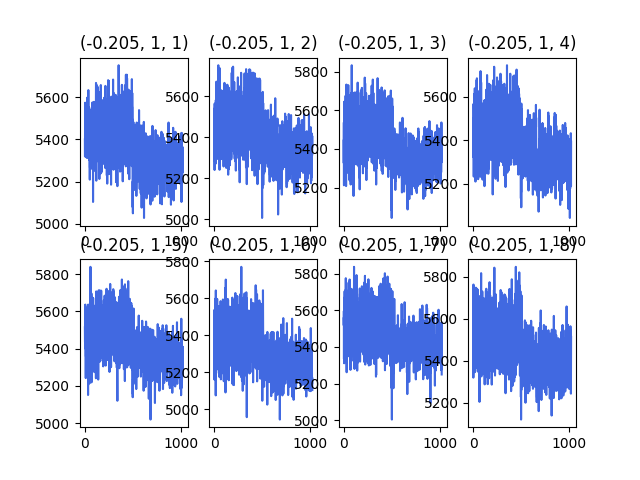
\includegraphics[width=0.6\linewidth]{plots_for_-0_027_all_channels.png}
    \caption{Данные для уровня -0.027, 1 канала, 2 ячейки}
\end{figure}\\
\begin{figure}[h!]
    \centering
    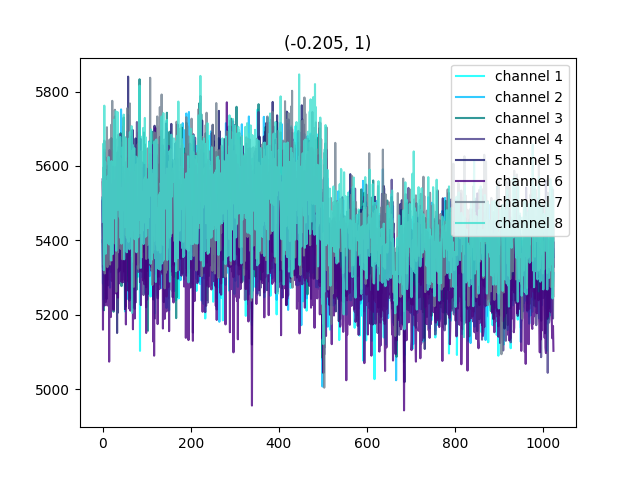
\includegraphics[width=0.6\linewidth]{all_channels_-0_027_fr_1.png}
    \caption{Данные для уровня -0.027, 1 канала, 2 ячейки}
\end{figure}\\
Видим по графикам, что в данных есть выбросы, их можно отсеять с помощью боксплота. На гистограмме ниже представлены данные до отсеивания выбросов и после:
\begin{figure}[h!]
    \centering
    \includegraphics[width=0.6\linewidth]{lvl_-0.027_ch_0_cell_10.png}
    \caption{Вид данных для $lvl = -0.027$, $ch = 0$, $cell = 10$ до и после отсеивания выбросов}
    \label{fig:enter-label}
\end{figure}
\newpage
\hspace{-0.5cm}\textbf{1. Оценки значений Y}\\
Для внешних оценок возьмем границы боксплота (после отсеивания выбросов берем минимум и максимум) с параметром k=1.5, а для внутренних 1-й и 3-й квартили:
\begin{figure}[h!]
    \centering
    \includegraphics[width=0.25\linewidth]{y_int-y_ext.png}
    \caption{Внешние и внутренние оценки для каждого файла}
\end{figure}\\
\begin{figure}[h!]
    \centering
    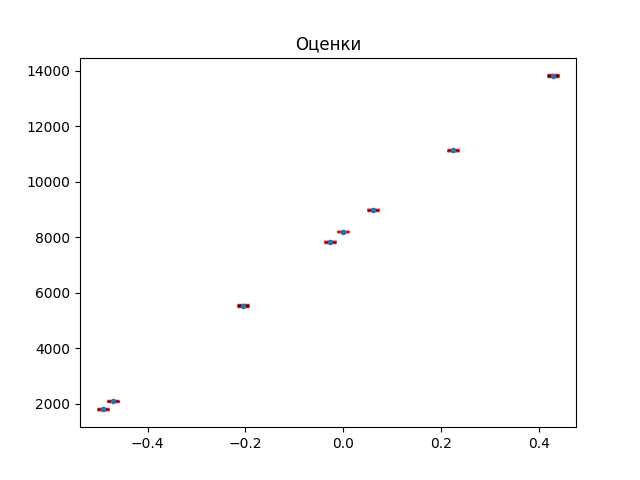
\includegraphics[width=0.45\linewidth]{visual_inners_externals_small.png}
        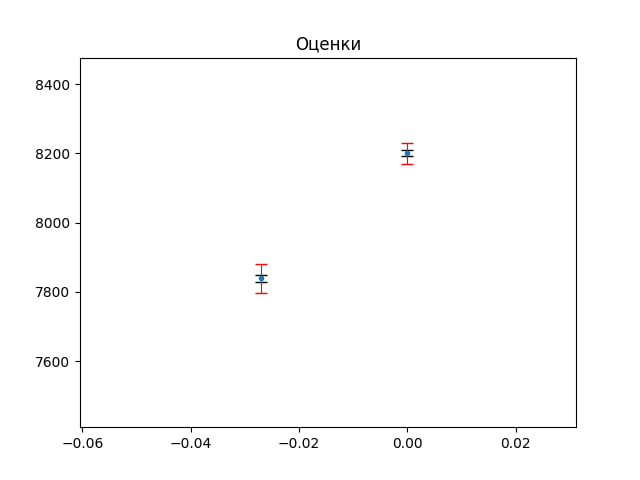
\includegraphics[width=0.45\linewidth]{visual_inners_externals_big.png}
    \caption{Внешние и внутренние оценки для каждого файла}
\end{figure}\\
\newpage
\hspace{-0.5cm}\textbf{1. Построение допускового множества}\\
Выберем для демонстрации работы алгоритма канал и ячейку - channel = 1, cell = 1023
\begin{figure}[h!]
    \centering
    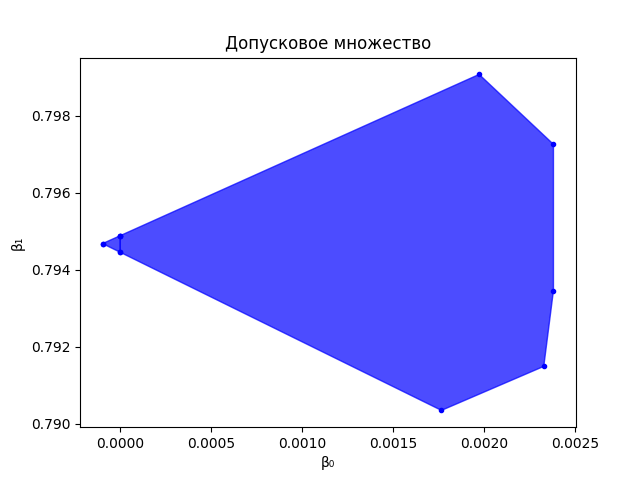
\includegraphics[width=0.75\linewidth]{tol-before-alg.png}
    \caption{Допусковое множество до раширения внутренних оценок до внешних}
\end{figure}\\
\hspace{-0.5cm}Видим, что на графике отображается только множество внешних оценок. Это говорит о том, что ИСЛАУ для неизвестных коэффициентов регресии несовместна. Для того, чтобы получить множество внутренних оценок, заменим строки системы с отрицательной невязкой (неомера уравнений будут номерами образующих распознающего функционала с отрицательным значением Tol'a)

\begin{figure}[h!]
    \centering
    \includegraphics[width=0.53\linewidth]{image.png}
    \caption{Результаты вычиселений для пустого допускового множества}
\end{figure}\\
\newpage
\hspace{-0.5cm}Расширяем внутренние оценки до внешних:
\begin{figure}[h!]
    \centering
    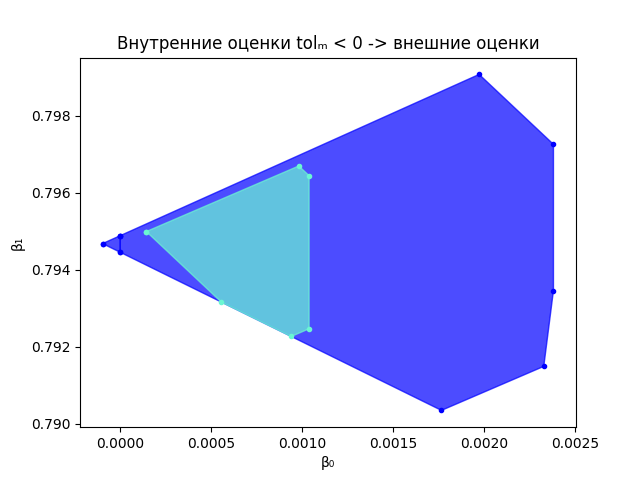
\includegraphics[width=0.65\linewidth]{tol-after-alg.png}
    \caption{Допусковое множество до раширения внутренних оценок до внешних}
\end{figure}
\begin{figure}[h!]
    \centering
    \includegraphics[width=0.53\linewidth]{image1.png}
    \caption{Результаты вычиселений для непустого допусскового множества}
\end{figure}\\
\newpage
\begin{figure}[h!]
    \centering
    \includegraphics[width=0.75\linewidth]{image2.png}
    \caption{Результаты вычисления коэффициентов}
\end{figure}
\begin{figure}[h!]
    \centering
    \includegraphics[width=0.4\linewidth]{image4.png}
    \includegraphics[width=0.4\linewidth]{image_.png}
    \caption{Результаты применения вычисленных коэффициентов к тренировочным данным}
\end{figure}
\newpage
\hspace{-0.5cm}\textbf{1. Коридор значений}\\
\begin{figure}[h!]
    \centering
    \includegraphics[width=0.75\linewidth]{Model_Set.png}
    \caption{Коридор значений}
\end{figure}
\begin{figure}[h!]
    \centering
    \includegraphics[width=0.75\linewidth]{Model_Set_big.png}
    \caption{Коридор значений (правый край)}
\end{figure}
\section{Выводы}
  В ходе выполнения лабораторной работы была реализована методика оценки
  параметров линейной регрессии на основе интервальных данных. Основные
  результаты включают в себя:

  \begin{itemize}
    \item Разработан алгоритм для нахождения внутренних и внешних оценок
      параметров линейной регрессии, что позволяет учитывать
      неопределённость в данных.
    \item Получены интервальные оценки параметров \( \beta_0 \) и
      \( \beta_1 \), которые демонстрируют диапазон возможных значений
      параметров регрессии.
    \item Построены коридоры совместных зависимостей, которые
      визуализируют интервальные решения и помогают в анализе устойчивости
      модели.
  \end{itemize}\\
  Результаты показывают, что предложенный подход позволяет более точно
  моделировать зависимости в данных, учитывая возможные вариации и ошибки.
  Это особенно полезно в приложениях, где точность измерений может
  варьироваться, и требуется надёжная оценка параметров модели.
\section{Литература}
\begin{enumerate}
    \item A.Н.Баженов. Интервальный анализ. Основы теории и учебные примеры. СПБПУ. 2020
    \item Официальная документация intvalpy: \url{https://intvalpy.readthedocs.io/ru/latest/#} 
    \item A.Н.Баженов., Н.В.Ермаков. Малоракурсная томография. Спб.: Политех-Пресс. 2023.  
\end{enumerate}

\end{document}